\pagebreak
\section{Ausschüttungspolitik}

\textbf{Verwendung der freien Cash Flows}:
\begin{center}
	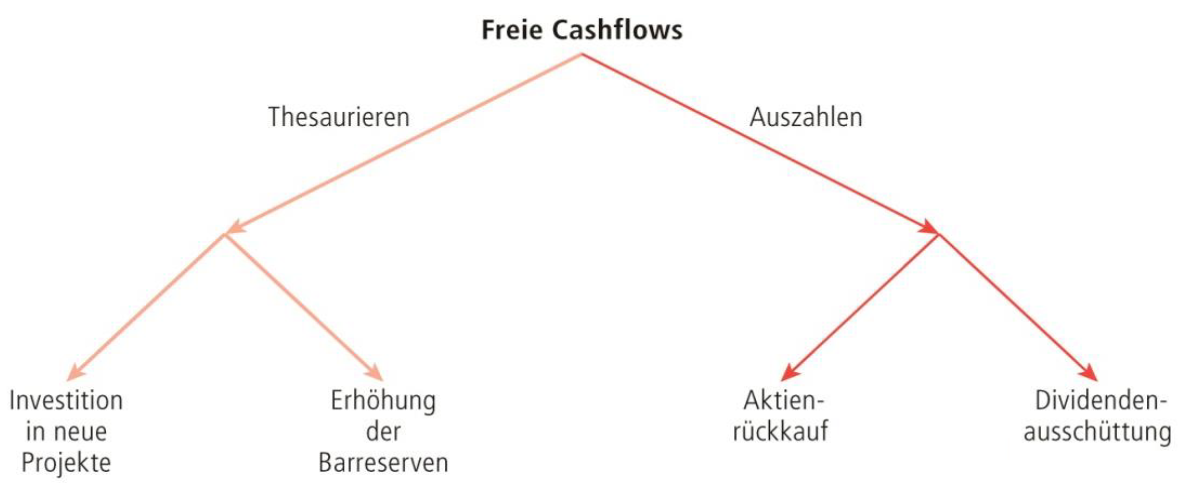
\includegraphics[width=0.7\textwidth]{images/fc.png}
\end{center}
Thesaurieren = Anhäufen, Horten\\

\textbf{Bemessung der Ausschüttung}:
\begin{itemize}
	\item Ausschüttungen von Dividenden orientieren sich am Jahresüberschuss
	\item Volumen der Aktienrückkäufe wird durch Hauptversammlung beschlossen
	\item Unvollkommenheiten der Kapitalmärkte beeinflussen Ausschüttungsstrategie $\rightarrow$ Aktienkurs reagiert auf Ankündigung einer Ausschüttung
	\item Bei vollkommenen Kapitalmarkt: Egal, ob Ausschüttungen in Form von Dividenden oder Aktienrückkäufen stattfinden (MM-Theorem)
\end{itemize}
\bigskip
\textbf{Ausschüttung vs. Thesaurierung}:
\begin{itemize}
	\item \textbf{Freie Cash Flows} (solche für die es keine Investitionen mit positivem Kapitalwert gibt) führen zu Agency-Kosten
	\item \textbf{Kapitalmarkt ist vollkommen}: Wenn alle Investitionen mit pos. Kapitalwert getätigt wurden, ist es egal, ob Überschuss thesauriert oder ausgezahlt wird
	\item \textbf{Kapitalmarkt ist unvollkommen}: Thesaurierung kann Kosten für künftige Kapitalbeschaffung reduzieren, erhöht aber Agency-Kosten
\end{itemize}
$\rightarrow$ Unternehmen sollten freie Cash Flows an die Eigentümer ausschütten\\

\textbf{Dividenden}: 
\begin{itemize}
	\item Können nicht von der Steuer abgesetzt werden
	\item Keine Zahlungsverpflichtungen $\rightarrow$ Führen nicht zur Insolvenz
	\item Auf perfekten Kapitalmärkte sinkt der Aktienkurs um die ausgezahlte Dividende
	\item Auf realen Märkten wird der Dividendenabschlag von der Marktentwicklung überlagert
	\item \textbf{Dividend Smoothing}: Dividenden haben \enquote{verbindlichen} Charakter gegenüber Aktionären $\rightarrow$ Langfristig möglichst stabile, geglättete Dividenden
	\item \textbf{Grund}: \textbf{Signalwirkung von Dividenden} $\rightarrow$ Dividendenveränderungen sind ein Signal bzgl. zukünftige Erwartungen des Unternehmens $\rightarrow$ Aktienmarkt reagiert positiv auf Dividendenerhöhung und negativ auf Dividendensenkungen
	\item \textbf{Dividend Catering}: Entscheidung eines Unternehmens, Dividenden zu zahlen, ist abhängig von der Nachfrage nach Ausschüttungen
\end{itemize}
\bigskip
\textbf{Modell der Dividendenpolitik nach Lintner}:
\begin{itemize}
	\item Annahme: langfristige Zielausschüttungsquote $d^*$
	\item Anpassungen der Dividenden an Gewinnänderungen verzögert, da Dividend Smoothing betrieben wird $\rightarrow$ Dämpfungsfaktor $\alpha$
	$$\Delta\text{Div}=\text{Div}_t-\text{Div}_{t-1}=\alpha(d^*\cdot\text{EPS}_t-\text{Div}_{t-1})\quad\text{mit EPS = Gewinn pro Aktie}$$

	Aus diesem Modell resultiert folgendes Regressionsergebnis:
	$$\Delta A=59,86+0,1524\cdot\text{EAT}-0,372\cdot A_{t-1}$$	
	mit $A=\text{Ausschüttung und EAT}=\text{Nachsteuergewinn}$
	\begin{itemize}
		\item Anpassungsparameter $\alpha=0,372$
		\item Ziel-Ausschüttungsquote $d^*= 0,1524/\alpha = 41\%$ 
	\end{itemize}
\end{itemize}
$\rightarrow$ Lintner-Modell liefert beschreibt das Ausschüttungsverhalten, es macht keine Aussage darüber, ob Gewinne ausgeschüttet werden sollten oder nicht\\

\textbf{Aktienrückkäufe}:
\begin{itemize}
	\item Unternehmen verwendet Barmittel, um eigene Aktien zurückzukaufen
	\item Kann für Aktionäre steuerlich vorteilhaft sein, wenn realisierte Kursgewinne niedriger besteuert werden als Dividenden
	\item Arten eines Aktienrückkaufs:
	\begin{itemize}
		\item \textbf{Open Market Repurchase}: Absicht, eigene Aktien zu erwerben, wird angekündigt, Rückkauf meist innerhalb eines Jahres, nicht alle
		annoncierten Aktien müssen aufgekauft werden
		\item \textbf{Tender Offer}: Fixes Übernahmeangebot mit Preispremium, Binnen einer speziellen Frist, Geeignet für größere Aktienpakete
		\item \textbf{Targeted Repurchase}: Direkte Adressierung eines Großaktionärs, Vermeidung von Preiseffekten auf illiquiden Märkten $\rightarrow$ Aktionäre fordern oft eine zusätzliche Prämie (\textbf{Greenmail})
	\end{itemize}
	\item Bilanzverkürzung bei Aktienrückkauf, Reduzierung der Anzahl umlaufender Aktien $\rightarrow$ Ergebnis je Aktie steigt
	\item \textbf{Ankündigungseffekt} von Aktienrückkäufen: Signal, dass das Unternehmen unterbewertet ist, Änderung der Kapitalstruktur (EK $\rightarrow$ FK), Ausschüttung von Free Cash Flow $\rightarrow$ Reduzieren vo Agency-Kosten
\end{itemize}
\bigskip
\textbf{Dividenden vs. Aktienrückkäufe}:
\begin{itemize}
	\item Dividenden sind meist mit einem höheren Steuersatz belegt als Kapitalgewinne, die ein Investor durch ein Aktienrückkauf erzielen kann
	\item \textbf{Dividend puzzle}: Dividenden bleiben trotz ihrer steuerlichen Nachteile ein weiterhin häufig verwendetes Mittel der Ausschüttungspolitik
	\item \textbf{Gründe}: Steuerarbitrage, Dividend Premium
\end{itemize}

\textbf{Steuerarbitrage}: Niedrig besteuerte Investoren kaufen Aktien vor dem Ex-Dividenden-Termin, erhalten Dividende ohne große Steuerlast und verkaufen hinterher

\textbf{Cum-Ex-Geschäfte}:
\begin{center}
	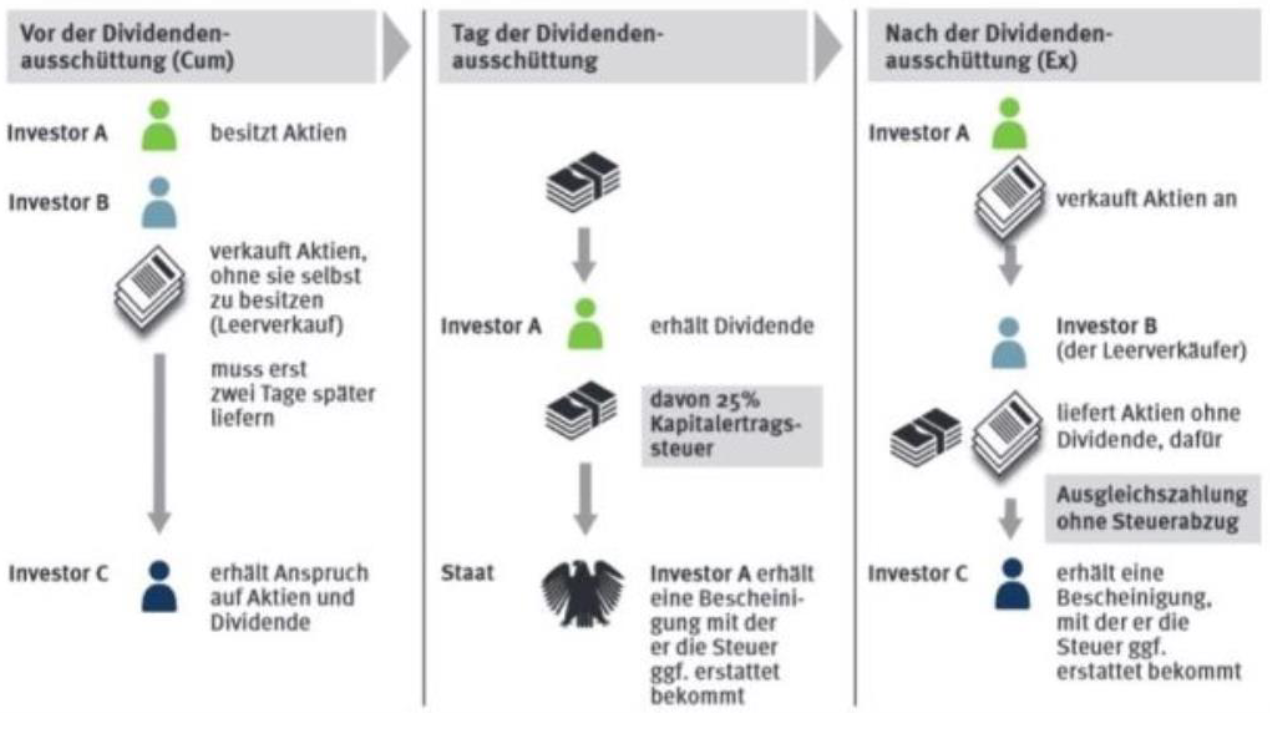
\includegraphics[width=0.8\textwidth]{images/cum-ex.png}
\end{center}
\pagebreak
\textbf{Cum-Cum-Geschäfte}:
\begin{center}
	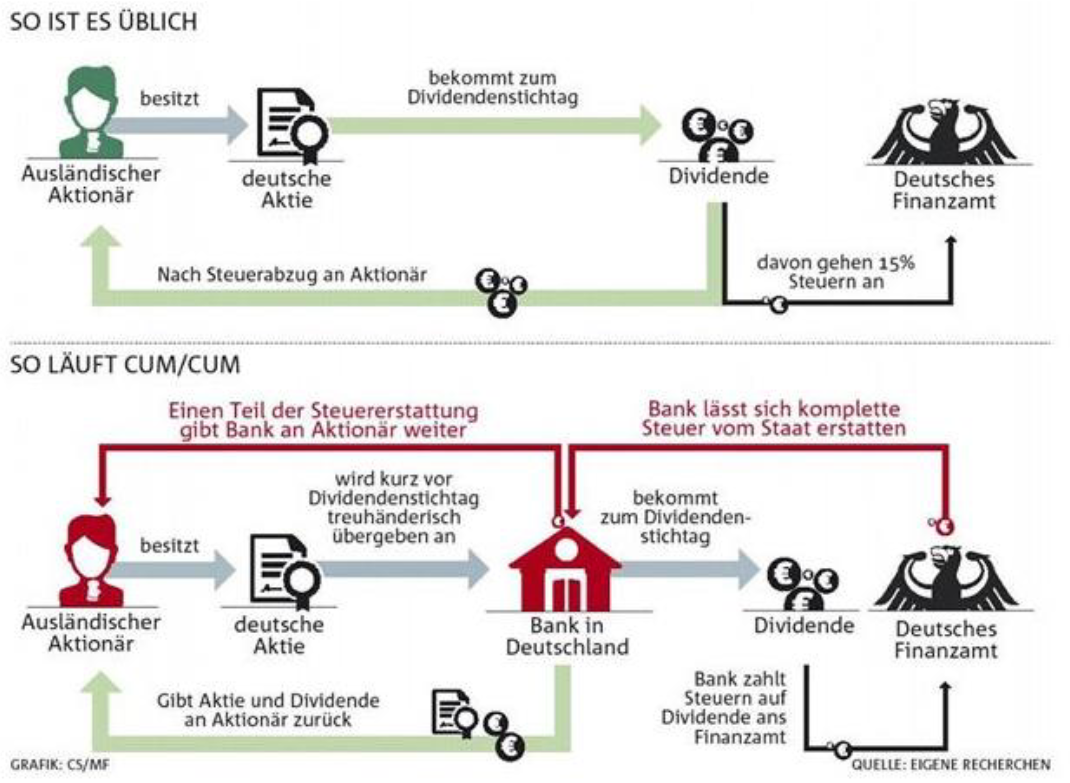
\includegraphics[width=0.7\textwidth]{images/cum-cum.png}
\end{center}
\bigskip
\textbf{Einflussfaktoren der Ausschüttungspolitik}:
\begin{itemize}
	\item Jahresüberschuss
	\item Gesetzliche, satzungs- und vertragsmäßige Restriktionen
	\item Steuerliche Rahmenbedingungen
	\item Ziel-Kapitalstruktur
	\item Liquiditätssituation und Finanzierungskosten
	\item Signalwirkung und Investorennachfrage
\end{itemize}
